\paragraph{La classe LogManagerViewModel}

\begin{minipage}
    {\linewidth}
    \centering
    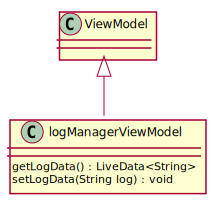
\includegraphics[width=0.80\linewidth]{../schemas/Conception_detaillee/classe_logManagerViewModel.pdf}
    \captionof{figure}{Diagramme de classe de LogManagerViewModel}
\end{minipage}

\subparagraph{Philosophie de conception \newline} 

\medspace

La classe LogManagerViewModel permet de faire le lien entre la vue du sniffer et les sources de données adjacentes. 

\subparagraph{Description structurelle \newline}

\medspace

\textbf{Attributs :}

N.A.

\textbf{Services offerts :}

\begin{itemize}
    \item \textbf{getLogData() : LiveData<String>} --- Opération qui a pour but de stocker des chaînes de caractères représentant les messages de trames. 
    \item \textbf{setLogData(log : String) : void} --- Opération qui permet de mettre à jour l'interface utilisateur en fonction des changements de logData. 
\end{itemize}
